\documentclass[tikz,border=5pt]{standalone}
\usepackage{amsmath}
\usepackage{xcolor}

% Uncomment for a Times-like look:
% \usepackage{newtxtext,newtxmath}

\colorlet{axiscol}{black}
\colorlet{curveUpper}{black}
\colorlet{curveLower}{gray!65}

\begin{document}
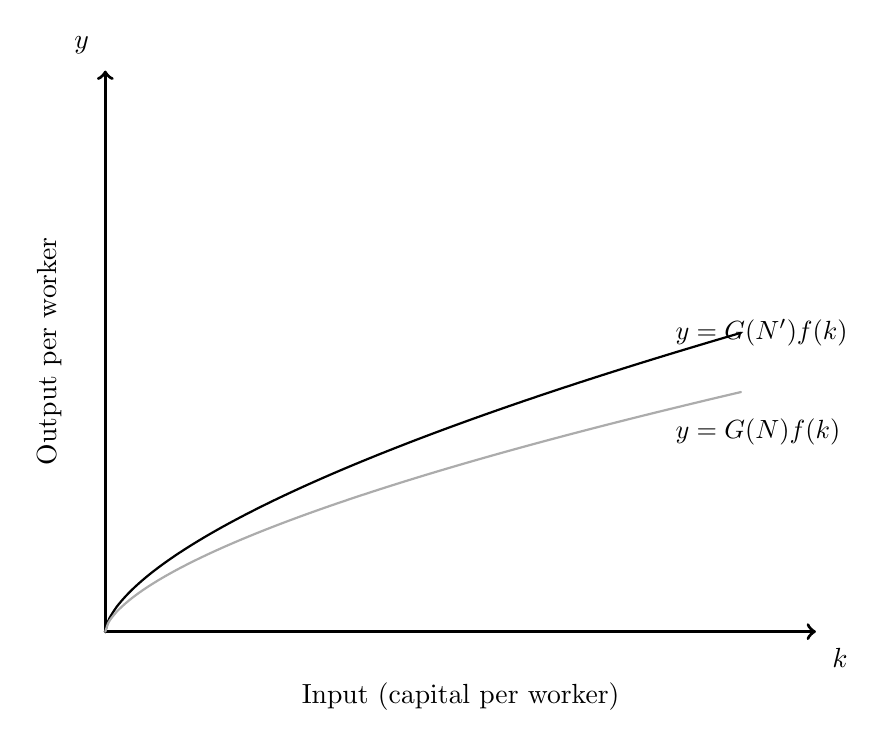
\begin{tikzpicture}[scale=0.95, line cap=round, line join=round]

  % Canvas limits
  \def\xmax{9.5}
  \def\ymax{7.5}

  % Function shape: diminishing returns (concave, increasing)
  % Adjust exponent (0<alpha<1) for curvature; scale factors for vertical position.
  \pgfmathdeclarefunction{f}{1}{\pgfmathparse{pow(max(#1,0),0.62)}}
  \def\GA{1.06} % upper curve scale = G(N')
  \def\GB{0.85} % lower curve scale = G(N)

  % Styles
  \tikzset{
    axis/.style={->, very thick, color=axiscol},
    curveU/.style={thick, color=curveUpper},
    curveL/.style={thick, color=curveLower}
  }

  % Axes
  \draw[axis] (0,0) -- (\xmax,0) node[below right=2pt] {$k$};
  \draw[axis] (0,0) -- (0,\ymax) node[above left=2pt] {$y$};

  % Axis captions
  \node[below] at (\xmax/2,-0.55) {Input (capital per worker)};
  \node[rotate=90] at (-0.75,\ymax/2) {Output per worker};

  % Curves
  \draw[curveU]
    plot[domain=0:\xmax-1, samples=220, smooth]
      (\x, {\GA * (f(\x))});
  \draw[curveL]
    plot[domain=0:\xmax-1, samples=220, smooth]
      (\x, {\GB * (f(\x))});

  % Labels for curves (adjust positions if needed)
  \path (\xmax-2, {\GA * f(\xmax-2)}) node[above right, scale=0.95] {$y = G(N')f(k)$};
  \path (\xmax-2, {\GB * f(\xmax-2)}) node[below right, scale=0.95] {$y = G(N)f(k)$};

\end{tikzpicture}
\end{document}